\section{Introduction}

Flutter has emerged as a crucial framework for mobile and web development, offering a range of advantages that make it a popular choice for cross-platform applications:
\begin{enumerate} 
    \item \textit{Widespread adoption}: Flutter has the highest number of users among cross-platform frameworks, making it a leading solution for multi-platform development. 
    \item \textit{Google support}: as an open-source framework backed by Google, Flutter benefits from regular updates, community contributions, and long-term stability. 
    \item \textit{Dart language}: Flutter uses Dart, a programming language similar to Java, making it easy to learn and adopt for developers familiar with object-oriented languages. 
    \item \textit{Extensive platform support}: Flutter provides a wide codebase solution, supporting development across multiple devices and platforms, including mobile (iOS, Android), web, and desktop. 
\end{enumerate}
Flutter's architecture can be understood through three distinct abstraction layers, each playing a key role in the app development process:
\begin{figure}[H]
    \centering
    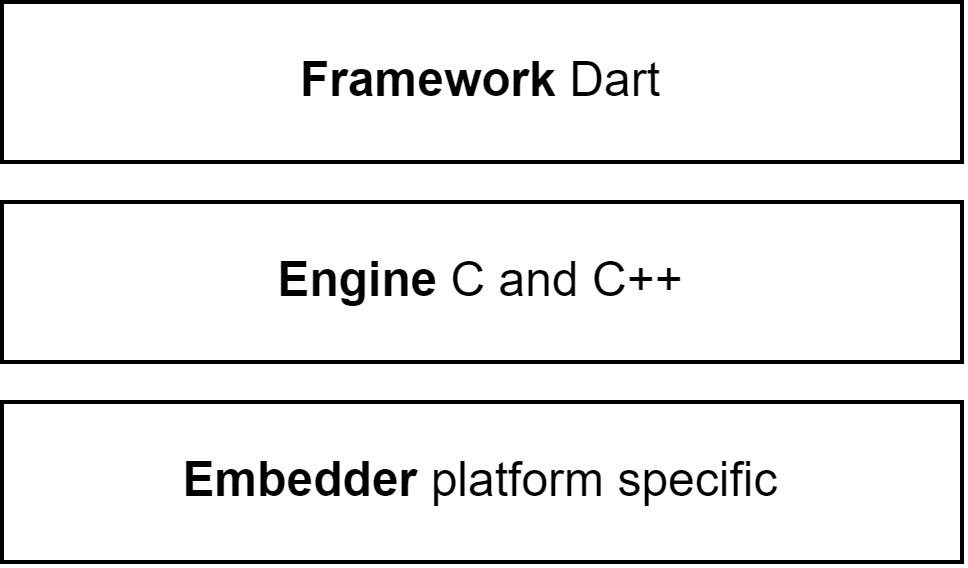
\includegraphics[width=0.65\linewidth]{images/flutter.png}
    \caption{Flutter architecture}
\end{figure}
The architecture consists of the following layers:
\begin{itemize}
    \item \textit{Embedder}: the embedder is responsible for integrating Flutter's source code into specific platforms, such as iOS, Android, or desktop environments. 
        This layer, developed by Google, ensures that Flutter can operate seamlessly across diverse platforms.
    \item \textit{Engine}: the engine manages the execution of the application on various devices, handling the compilation process and ensuring that the code is optimized for each target platform.
    \item \textit{Framework}: written in Dart, the framework is the layer that developers interact with the most. 
        It provides the tools and libraries necessary to create the application's user interface, manage state, and implement core functionality.
\end{itemize}